\documentclass[tikz]{standalone}

\usepackage{amsmath}
\usepackage{unicode-math}
\usepackage{mathtools}
\usepackage{derivative}

\setmainfont{Stix Two Text}
\setmathfont{Stix Two Math}

\usetikzlibrary{arrows.meta,fit,positioning}

\renewcommand{\familydefault}{\sfdefault}

% prefix equation numbers with section number
\numberwithin{equation}{section}

\DeclarePairedDelimiter{\ceil}{\lceil}{\rceil}
\DeclarePairedDelimiter{\floor}{\lfloor}{\rfloor}
\DeclarePairedDelimiter{\abs}{\lvert}{\rvert}
\DeclarePairedDelimiter{\norm}{\lVert}{\rVert}
\DeclarePairedDelimiter{\bra}{\langle}{\rvert}
\DeclarePairedDelimiter{\ket}{\lvert}{\rangle}
\DeclarePairedDelimiter{\expval}{\langle}{\rangle}
\DeclarePairedDelimiter{\norder}{\mathcolon}{\mathcolon}
\DeclarePairedDelimiter{\anorder}{\typecolon}{\typecolon}
	
\newcommand{\laplace}{\mbfnabla^2}
\newcommand{\trans}{{\scriptscriptstyle\mathsf{T}}}

\newcommand{\vdot}{\cdot}
\newcommand{\vcross}{\vectimes}
\newcommand{\vb}[1]{\symbfup{#1}}
\newcommand{\vu}[1]{\hat{\vb{#1}}}
\newcommand*\dd[2][\relax]{\mathop{\ifx\relax#1\odif{#2}\else \odif[order={#1}]{#2}\fi\,}}

\newcommand{\vacuum}{\ket*{\vb{0}}}

\DeclareMathOperator{\trace}{Tr}
\DeclareMathOperator{\sinc}{sinc}

\AtBeginDocument{
	\let\Re\relax
	\let\Im\relax
	\DeclareMathOperator{\Re}{Re}
	\DeclareMathOperator{\Im}{Im}

	\renewcommand{\div}{\mathop{\mbfnabla\vdot}}
	\newcommand{\curl}{\mathop{\mbfnabla\vectimes}}
}

\DeclarePairedDelimiterX{\comm}[2]{[}{]}{#1,#2}

\DeclarePairedDelimiterX{\braket}[2]{\langle}{\rangle}{#1\delimsize\vert#2}
\DeclarePairedDelimiterX{\ketbra}[1]{\lvert}{\rvert}{#1\rangle\delimsize\langle#1}



\usetikzlibrary{arrows.meta}
\usetikzlibrary{decorations.pathmorphing}

\begin{document}
	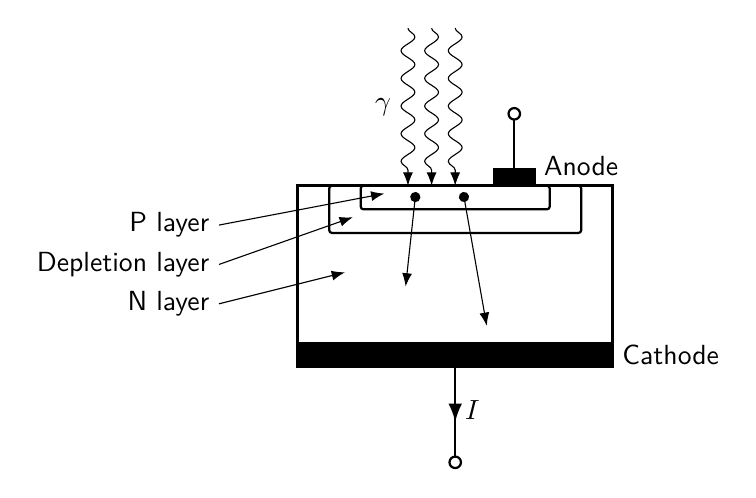
\begin{tikzpicture}[
		photon/.style={-Latex, decorate, decoration={snake, post length=1mm}},
		electron/.style={Circle-Latex},
	]
		\draw[very thick] (0,0) rectangle ++(4,2);
		\draw[very thick, fill] (0,0) rectangle ++(4,-0.3);
		\draw[very thick, fill] (2.5,2) rectangle ++(0.5,0.2);
	
		\draw (4,-0.15) node[right] {Cathode};
		\draw (3.6,2) node[above] {Anode};
		\draw[thick, -{Circle[open]}] (2.75,2) -- ++(0,1);
		
		\draw[thick, rounded corners=1pt] (0.8,2) rectangle ++(2.4,-.3);
		\draw[thick, rounded corners=1pt] (0.4,2) rectangle ++(3.2,-.6);
		
		\draw[-Latex] (-1,1) node[left] {Depletion layer} -- (0.7,1.6);
		\draw[-Latex] (-1,1.5) node[left] {P layer} -- (1.1,1.9);
		\draw[-Latex] (-1,0.5) node[left] {N layer} -- (0.6,.9);

		\draw[photon] (1.4,4) -- ++(0,-2) node[midway, left, xshift=-0.1cm] {$\gamma$};
		\draw[photon] (1.7,4) -- ++(0,-2);
		\draw[photon] (2,4) -- ++(0,-2);
		\draw[electron] (2.1,1.92) -- ++(0.3,-1.7);
		\draw[electron] (1.5,1.92) -- ++(-0.13,-1.2);
		
		\draw[thick, -Latex] (2,0) -- ++(0,-1) node[right, yshift=0.15cm] {$I$};
		\draw[thick, -{Circle[open]}] (2,-0.6) -- ++(0,-1);
	\end{tikzpicture}
\end{document}
